\section{Collecte automatisée}
\begin{tcolorbox}[title=Les déchets des uns...]
On dit que les rues du Web sont pavées de données qui n'attendent que la collecte... mais la quantité de déchets qu'on y retrouve est surprenante. \\[-0.6cm]
\begin{flushright}
-- Patrick Boily, 2020
\end{flushright}
\end{tcolorbox}
\noindent Les façons dont les données sont \textbf{partagées}, \textbf{recueillies} et \textbf{publiées} ont bien changé au cours des dernières années en raison de l'omniprésence du \textit{World Wide Web}. Les \textbf{entreprises privées}, les \textbf{gouvernements} et les \textbf{utilisateurs individuels} publient et partagent toutes sortes de données et d'informations. À chaque instant, des mécanismes engendrent de grandes quantités de données.
%Il fut un temps, dans un passé récent, où la rareté et l'inaccessibilité des données constituaient un problème pour les chercheurs et les décideurs. Ce n'est \textbf{définitivement} plus le cas.  
\newl L'abondance des données pose toutefois certains problèmes, notamment en ce qui concerne 
\begin{itemize}[noitemsep]
\item des masses de données enchevêtrées, et 
\item des méthodes traditionnelles de collecte et d'analyse de données qui ne sont plus à la hauteur en raison de leur manque d'efficacité.
\end{itemize}
La popularité et la puissance croissantes des \textbf{logiciels libres}, tels que \text{R} et \text{Python} (dont le code source peut être inspecté, modifié, et amélioré par quiconque), rendent la collecte automatisée de données très attrayante. 

Mais attention: les modules et les librairies de code deviennent \textbf{désuets} en un clin d'œil. Si l'analyste est incapable (ou refuse) de \textbf{maintenir leur programme d'extraction et d'analyse} et de \textbf{surveiller les sites} desquels les données sont extraites, le choix du logiciel ne fera pas, en fin de compte, une grande différence. 
\newpage\noindent
Alors pourquoi prendre la peine d'automatiser la collecte des données? Voici quelques considérations courantes:
\begin{itemize}[noitemsep]
    \item la faiblesse des ressources financières;
    \item le manque de temps ou le désir de recueillir les données manuellement;
\item orte le désir de travailler avec des sources de données actualisées de haute qualité, et  
\item la nécessité de documenter le processus analytique du début (collection) jusqu'à la fin (publication).
\end{itemize} 
La collecte manuelle, en revanche, tend à être encombrante et sujette aux erreurs; les approchess non reproductibles sont également sujettes à des risques accrus de ``mort par ennui'', alors que les solutions programmattiques sont généralement plus fiables, reproductibles, rapides, et produisent des données de meilleure qualité (en supposant que des données cohérente existent au départ). 
\subsection{Liste de contrôle pour la collecte automatisée} Cela dit, le \textbf{raclage de la toile} (web scraping) n'est pas toujours recommandé. En premier lieu, il est possible qu'aucune source de données en ligne et librement accessible ne réponde aux besoins de l'analyse, auquel cas on devrait privilégier une approche d'échantillonnage. \par Cependant, si la réponse à la plupart des questions suivantes est positive, une approche automatisée peut s’avérer être un choix judicieux.
\begin{itemize}[noitemsep]
\item Est-il nécessaire de répéter la tâche de façon périodique (par exemple pour mettre à jour une base de données)?
\item Est-il nécessaire que d'autres analystes soient en mesure de reproduire le processus de collecte?
\item Des sources de données en ligne sont-elles fréquemment utilisées?
\item La tâche est-elle non triviale en termes de portée et de complexité?
\item Si la tâche peut être effectuée manuellement, les ressources financières nécessaires manquent-elles?
\end{itemize}
L'objectif en est simple: la collecte automatique de données devrait permettre d'obtenir des données non structurées (ou non triées), à un prix raisonnable.
\subsection{Consid\'erations d'ordre éthique} Nous nous penchons à présent sur une question brûlante: les données disponibles en ligne sont-elles vraiment libres? 
\par Un \textbf{spider} est un programme qui parcourt rapidement le web à la recherche de données. Il s'aute d'une page à l'autre, en s'emparant de tout leur contenu. Le \textbf{raclage} (scraping), quant a lui, consiste à recueillir des renseignements spécifiques sur des sites  spécifiques: en quoi ces deux concepts sont-ils différents? 
\begin{quote}``Le raclage implique intrinsèquement la \textbf{copie} d’information; l'une des revendications les plus évidentes contre les grattoirs est donc  la violation des droits d'auteur.'' \cite{DC_MRMN}\end{quote}
Que peut-on faire pour minimiser le risque? 
\begin{itemize}[noitemsep]
\item travailler de manière aussi transparente que possible;
\item documenter les sources de données à tout moment;
\item remettre le mérite à ceux qui ont collecté et publié les données au départ;
\item demander l'autorisation de reproduire les informations (si vous ne les avez pas recueillies) et, surtout
\item ne commettre aucun acte illégal.
\end{itemize}
Les tribunaux n'ont pas encore trouvé leur rythme dans ce dossier (consulter, par exemple, \textit{eBay} vs \textit{Bidder's Edge}, \textit{Associated Press} vs \textit{Meltwater}, \textit{Facebook} vs \textit{Pete Warden}, etc. \cite{DC_M}). Il y a plusieurs questions juridiques \`a eétudier, mais il semble en général que les grandes entreprises/organisations sortent généralement victorieuses de ces batailles légales. \par La question est floue par ce qu’il n’est pas évident de différentier les actions de grattage illégales de celles qui sont légales. Il y a des lignes directrices approximatives: la republication de contenu à des fins commerciales est considérée comme plus problématique que le téléchargement de pages pour la recherche et l'analyse, par exemple. Le fichier \texttt{robots.txt} (``Robots Exclusion Protocol'', cf.\@ Figure~\ref{fig:robots}) indique aux gratteurs quelles informations peuvent être recueillies sur le site avec le consentement de leur auteur -- au minimum, il faut en tenir compte, quoique cela n'offre pas une protection absolue.
\begin{figure}[t]
\centering
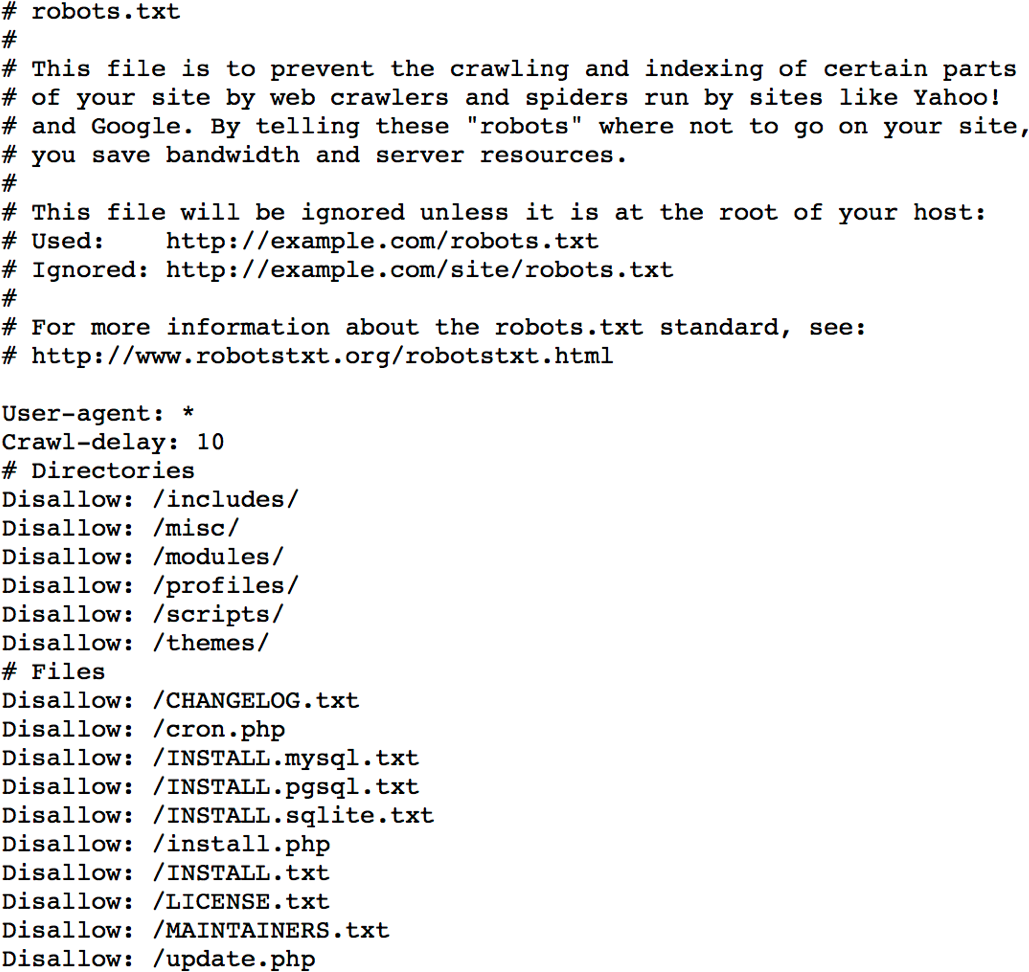
\includegraphics[width=0.50\textwidth]{Images/CQADS_robots.png}
\caption{Fichier \texttt{robots.txt} du site  \newhref{cqads.carleton.ca}{cqads.carleton.ca}.}\hrule\label{fig:robots}
\end{figure}
\afterpage{\FloatBarrier}
\newl Un bon programme de grattage doit 1) se comporter ``convenablement'', 2) fournir des données utiles, et 3) être efficace, dans cet ordre. En cas de doute, contactez les propriétaires du site afin de vérifier s'ils accordent l'accès aux bases de données ou aux fichiers. 
\newpage\noindent Notons finalement l'importance de suivre les \textbf{règles de bienséance} du grattage:
\begin{enumerate}[noitemsep]
    \item \textbf{demeurer identifiable};
    \item \textbf{réduire le trafic} -- accepter les fichiers comprimés, vérifier qu'un fichier a été modifié avant d'y accéder à nouveau, ne récupérer que les parties essentielles;
    \item \textbf{ne pas déranger le serveur avec des requêtes multiples} -- de nombreuses requêtes par seconde peuvent entraîner des pannes de serveur, ce qui peut mener les webmestres à vous bloquer si votre gratteur est trop gourmand (quelques requêtes par seconde suffisent);
    \item \textbf{écrire des grattoirs efficaces et polis} -- il n'y a aucune raison de gratter les pages quotidiennement ou de répéter la même tâche sans cesse… il est préférable de sélectionner des ressources spécifiques et de laisser le reste intact. 
\end{enumerate}
\subsection{Qualité des données de la toile} Le question de la qualité des données est incontournable. Il n'est pas rare de voir des organisations dépenser des milliers de dollars en collecte de données (automatique ou manuelle) mal concue pour ensuite insister que leurs analystes se servent de données défectueuses puisque ce sont les seules données disponibles. \par Ce problème peut être escamoté dans une certaine mesure lorsque les analystes participent aussi à la collecte des données:
\begin{itemize}[noitemsep]
    \item Quel type de données est le mieux adapté pour répondre à aux question de l'organisation?
    \item Les données disponibles sont-elles de qualité suffisante pour donner des reponses utiles aux questions du client?
    \item les informations disponibles sont-elles systématiquement erronées?
\end{itemize}
Sur la toile, les données peuvent provenir de \textbf{sources directes} (un tweet ou un article d'actualité), ou de \textbf{sources indirectes} (copiées d'une source hors ligne ou grattées à partir d’un autre site, ce qui peut rendre leur retraçage difficile). Le \textbf{recoupement de données} (``cross-referencing’’) est une pratique courante lorsqu’on compose avec des données secondaires.  \par La qualité des données dépend également de leur \textbf{usage} et des \textbf{objectifs} d'analyse. Par exemple, 
un échantillon de tweets recueilli un jour quelconque peut être utilisé afin d'analyser l'utilisation de ``hashtags'' spécifiques, mais cet ensemble de données peut s’avérer pratiquement inutile si l’échantillon est recueilli jour d'élection fédérale (en raison du \textbf{bias de collecte}).
\newl Un exemple peut aider à décortiquer les pièges et les défis. Supposons qu'un client souhaite savoir, grâce à une enquête téléphonique typique, ce que les gens pensent d'une nouvelle éplucheuse de patate.  Une telle approche comporte un certain nombre de risques:
\begin{itemize}[noitemsep]
\item\textbf{échantillon non représentatif} -- l'échantillon sélectionné peut ne pas représenter la population visée;
\item\textbf{non-réponse systématique} -- les gens qui n'aiment pas les enquêtes télépho\-ni\-ques peuvent être moins (ou plus) susceptibles d'aimer la nouvelle  éplucheuse;  
\item\textbf{erreur de couverture} -- les gens sans ligne télépho\-ni\-que fixe ne sont pas rejoignables, et \item\textbf{erreur de mesure} -- les questions de l'enquête peuvent ne pas fournir l'information requise.
\end{itemize}
Les solutions classiques à ces problèmes nécessitent le recours à l'échantillonnage, au design de questionnaires, %aux enquêtes omnibus, à des systèmes de récompense, 
etc. Ces solutions peuvent s’avérer  \textbf{coûteuses} et \textbf{inefficaces}. L’utilisation de ``\textbf{proxies}'’ peut aussi être utile -- il s’agit d'indicateurs fortement liés à la popularité d'un produit, telles les statistiques de vente sur un site web commercial. 
\par Le classement des éplucheuse sur \texttt{Amazon.ca} (ou un site web similaire) peut, en fait, dresser un portrait bien plus complet du marché des éplucheuses que ne pourrait le ferait une enquête traditionnelle (en supposant, bien sûr, que l’on fait confiiance à ce dernier). L’information recherchée pourrait donc être obtenue en élaborant un scraper compatible avec l'\textbf{interface de programmation} (API) d'Amazon afin de  recueillir les données appropriées.\newl Il va de soit que cette approche peut également poser certains problèmes: 
\begin{itemize}[noitemsep]
\item \textbf{représentativité} des \textbf{produits listés} -- est-ce que les éplucheuses sont toutes répertoriées? Si ce n'est pas le cas, est-ce parce que ce site web ne les vend pas? Y a-t-il une autre raison?
\item \textbf{représentativité} des \textbf{clients} -- y a-t-il des groupes spécifiques qui achètent (ou non) de produits en ligne? Y a-t-il des groupes spécifiques qui achètent sur des sites spécifiques? Y a-t-il des groupes spécifiques qui laissent (ou non) des critiques de produits? 
\item \textbf{fiabilité} des clients et des critiques -- comment dis\-tin\-gue-t-on les fausses critques des critiques réelles?
\end{itemize}
Le scraping est généralement bien adapté à la collecte de données sur les produits, mais il existe plusieurs situations pour lesquelles il est nettement plus difficile d'imaginer où trouver des données en ligne: quelles données pourriez-vous collecter en ligne afin de mesurer la popularité d'une politique gouvernementale, par exemple? 
\subsection{Technologies du web: premiers pas}
En ligne, les données sont retrouvées sous forme de \textbf{textes}, de \textbf{tableaux}, de \textbf{listes}, de \textbf{liens} et autres structures, mais elles ne sont pas présentées dans les fureteurs de la même manière qu'elles sont stockées en HTML/XML. De plus, lorsque les pages web sont \textbf{dynamiques}, il y a un "coût" associé à la collecte automatisée. Par conséquent, une connaissance de base du web et de ses technologies est cruciale. Des renseignements sont facilement accessibles en ligne (cf.\@ références) et dans \cite{DC_M,DC_MRMN}.\newpage\noindent Il existe trois domaines d'importance pour la collecte de données sur le web:
\begin{itemize}[noitemsep]
\item les technologies de \textbf{diffusion de contenu} (HTTP, HTML/XML, JSON, texte brut, etc.);
\item les technologies d'\textbf{extraction d'information} (Python, R, XPath, parser JSON, Beautiful Soup, Selenium, regexps, etc.), et 
\item tles echnologies de \textbf{stockage des données} (R, Python, SQL, formats binaires, formats de texte brut, etc.).
\end{itemize}
Le contenu d'une page Web se répartit en trois grandes catégories: le langage de balisage hypertexte (HTML; utilisé pour le contenu et le code web), les feuilles de style en cascade (CSS; utilisé pour le style des pages web) et le JavaScript (JS; utilisé pour l'interactivité avec la page web). En quelque sorte, la partie HTML est la plus fondamentale; c'est en comprenant la structure arborescente des documents HTML, par exemple, qu'on apprend à utiliser pleinement la \textbf{boîte à outils de grattage}. 
\subsection{Boîte à outils de grattage de la toile}
Nous constatons par expérience qu'un certain nombre d'outils peuvent faciliter le processus de collecte automatisé des données, notamment les \textit{outils de développement} (``Developer Tools''), \textit{XPath}, \textit{Beautiful Soup}, \textit{Selenium}, et les \textit{expressions régulières} (``regexps''). 
\newl Les \textbf{outils de développement} affichent la correspondance entre le code HTML d'une page et la version présentée par le navigateur (cf la Figure~\ref{fig:erb} en exemple). Contrairement à l'option ``View Source'', les outils de développement affichent la version \textit{dynamique} du contenu HTML (c'est-à-dire que le code HTML est affiché avec toutes les modifications apportées par JavaScript depuis la première réception de la page). \newl L'inspection des différents éléments d'une page et la découverte de leur emplacement dans le fichier HTML est un étape \textbf{cruciale} afin d'obtenir un grattage efficace: 
\begin{figure*}[t]
\centering
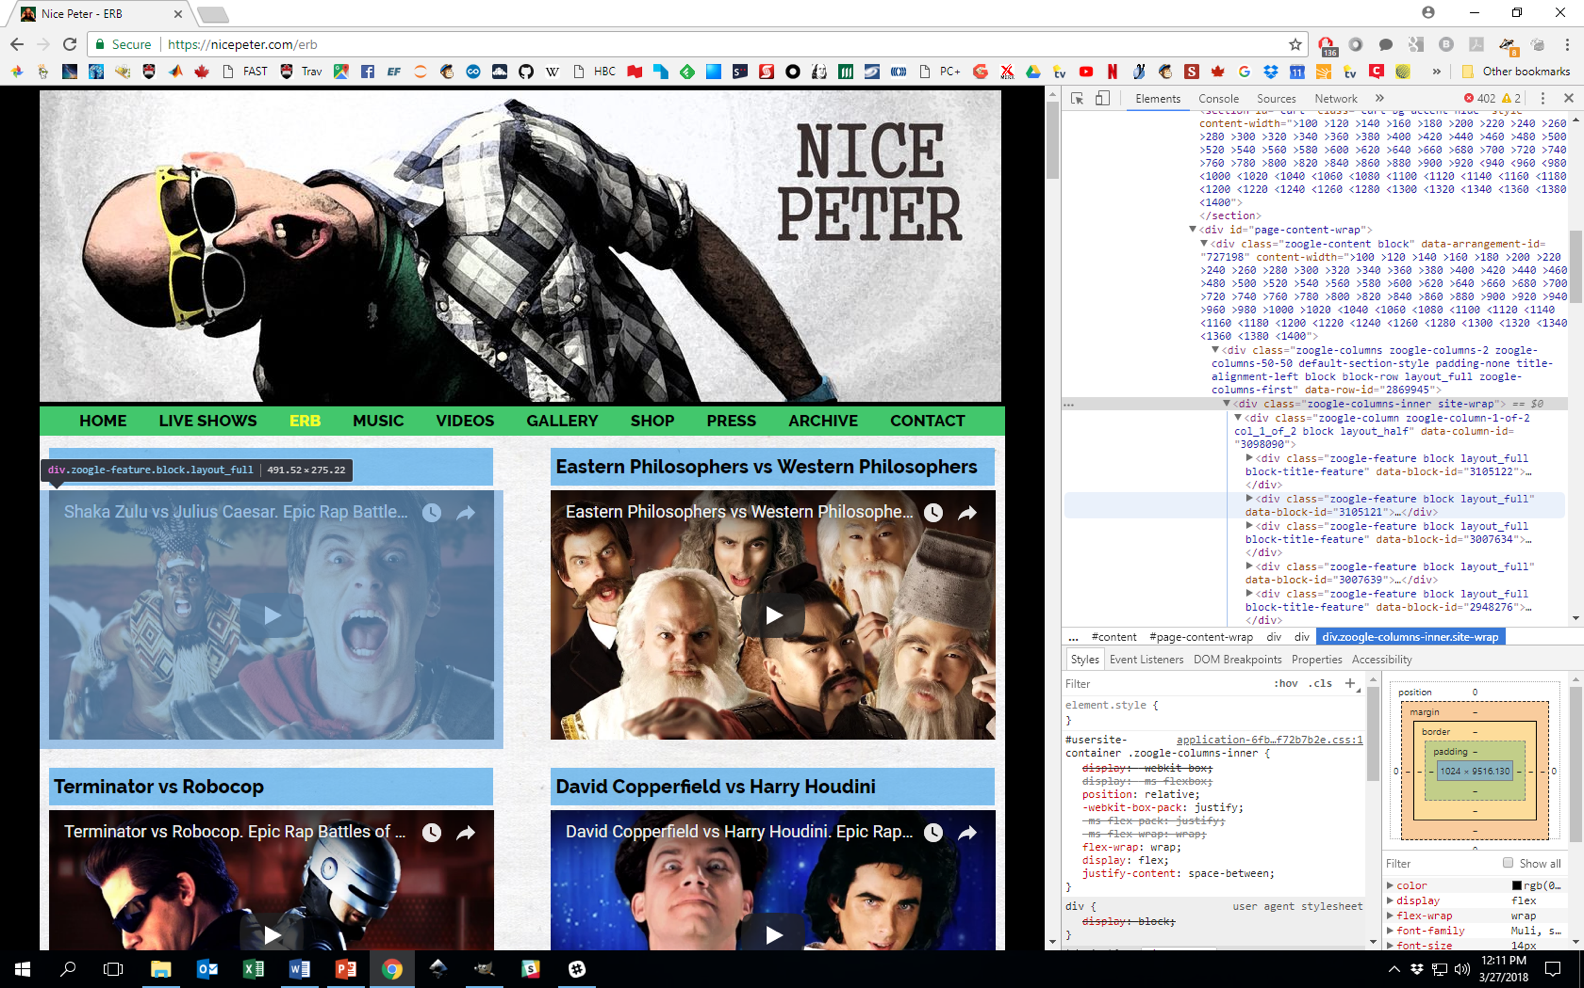
\includegraphics[width=0.65\textwidth]{Images/erb.png}
\caption{\small Inspection des éléments de la page YouTube  \newhref{https://nicepeter.com/erb}{https://nicepeter.com/erb} à l'aide des \textit{Developer Tools} de Chrome.} \hrule\label{fig:erb}
\end{figure*}
\begin{itemize}[noitemsep]
\item \textbf{Firefox} -- cliquer sur la page avec le bouton droit de la souris $\to$ ``Inspect Element''
\item \textbf{Safari} -- Safari $\to$ ``Preferences'' $\to$ ``Advanced'' $\to$ ``Show Develop Menu in Menu Bar'', et ensuite ``Develop'' $\to$ ``Show Web Inspector''
\item \textbf{Chrome} --  cliquer sur la page avec le bouton droit de la souris $\to$ ``Inspect''
\end{itemize}
\textbf{XPath} est un langage de requête  que l'on utilise afin de sélectionner des informations spécifiques dans des documents balisés tels que HTML, XML, etc. Avant que cela puisse être fait, les informations stockées dans un document balisé doivent être converties (``parsed'') dans un format adapté au traitement et à l'analyse statistique; le module XML implémente un tel ``parsing'' en R, par exemple. Le processus est simple; il suffit de: 
\begin{enumerate}[noitemsep]
\item préciser les données d'intérêt;
\item les situer dans un document spécifique, pour ensuite 
\item adapter une requête au document afin d'y extraire les informations souhaitées.
\end{enumerate}
Les requêtes XPath nécessitent à la fois un \textbf{chemin} et un \textbf{document} à rechercher; les chemins consistent en un mécanisme d'adressage hiérarchique (succession de nœuds, séparés par des barres obliques (``/''), tandis qu'une requête prend la forme \small\texttt{xpathSApply(doc,path)}\normalsize: par exemple,
\footnotesize\texttt{xpathSApply(parsed\_doc,``/html/body/div/p/i'')}\normalsize \\ trouve toutes les balises \texttt{<i>} se retrouvant sous une balise \texttt{<p>}, elle-m\^eme se situant sous une balise \texttt{<div>} dans le ``\texttt{body}'' du fichier \texttt{html} du document \texttt{parsed\_doc} (consultez \cite{DC_MRMN} pour une introduction plus étoffée). 
\newl On peut utiliser les \textbf{expressions régulières} pour réaliser l'objectif principal du grattage du web, qui est d'extraire des informations pertinentes parmi une multitude de données. \`A m\^eme ces données, pour la plupart non structurées, se cachent des \textbf{éléments systématiques} qui peuvent être employés afin de faciliter le processus d'automatisation, en particulier si des méthodes quantitatives seront éventuellement appliquées aux données raclées. Les structures systématiques comprennent des numéros, des noms (pays, etc.), des adresses (courrier, e-mail, URL, etc.), des chaînes de caractères spécifiques, etc. Les expressions régulières (regexps) sont des séquences abstraites de chaînes de caractères qui correspondent à des modèles concrets récurrents dans le texte; elles permettent l'extraction systématique des composantes d'information contenues  dans le texte brut, le HTML et le XML. Des exemples illustrant les principaux concepts sont présentés dans le \textit{Jupyter Notebooks} ci-joint. %showcased in Section~\ref{sec:docs}. 
\newl \textbf{Beatiful Soup} est un module Python qui permet d'extraire des données de fichiers HTML et XML. Il analyse les fichiers HTML (même ceux qui sont endommagés). Beautiful Soup ne se contente pas de convertir le mauvais HTML en code X/HTML valide; il permet \'egalement à un utilisateur d'ins\-pec\-ter la structure HTML (corrig\'ee) qu'il produit dans son ensemble, de manière programmatique. La \textbf{soupe} qui en résulte est une API qui permet de \textbf{parcourir}, \textbf{rechercher}, et \textbf{lire} les éléments du document. Elle fournit essentiellement des moyens de navigation, de recherche et de modification \textbf{idiomatique} de l'arbre d'analyse du fichier HTML, ce qui permet de gagner un temps considérable.
\par Par exemple, \texttt{soup.find\_all('a')} trouve et affiche toutes les paires de balises \texttt{<a ...> ... </a>}  (avec  attributs et contenu) se trouvant dans la soupe \texttt{soup}, tandis que \begin{quote}\texttt{for link in soup.find\_all('a'):}\newline \texttt{\ \ \ \ print(link.get('href')}
\end{quote} produit les adresses URL trouvées \'a m\^eme ces paires de balises. La documentation de Beautiful Soup fournit de nombreux exemples \cite{DC_S2}. 
\newpage\noindent\textbf{Selenium} est un outil Python utilisé pour automatiser les interactions avec des fureteurs.  On l'utilise principalement à des fins de ``testing'', mais on s’en sert également pour l'extraction de données. Il permet à l'utilisateur d'ouvrir un navigateur et d'agir ``naturellement’’, c’est-à-dire comme le ferait un être humain:
\begin{itemize}[noitemsep]
    \item en cliquant sur les boutons;
\item en saisissant des informations dans les formulaires;
\item en recherchant des informations spécifiques sur une page, etc.
\end{itemize}
Selenium requiert un ``driver’’ d'interface avec le navigateur choisi. Firefox, par exemple, utilise \texttt{geckodriver}. Les autres navigateurs soutenus ont leurs propres drivers (cf \cite{DC_S_E}).

Selenium contrôle automatiquement un navigateur dans son ensemble, y compris le ``rendering'' des documents web et l'exécution de code JavaScript, ce qui est utile pour les pages dont le contenu dynamique ne se retrouve pas dans la version standard de HTML. Selenium peut programmer des actions comme "cliquez sur ce bouton" ou "tapez ce texte" pour donner accès au HTML dynamique ou à l'état actuel de la page, du genre de ce qui se passe avec les outils de développement (mais le processus peut désormais être entièrement automatisé). Pour plus d'informations, voir \cite{DC_S,DC_S2}.
\newl 
Nous terminons cette section par un bref résumé du \textbf{processus décisionnel relatif à la collecte automatisée de données} \cite{DC_MRMN,DC_M}: 
\begin{enumerate}
    \item il faut bien savoir de \textbf{quel type d'information le client a besoin}, que ce soit \textbf{spécifique} (e PIB des pays de l'OPEC au cours des 10 dernières années, les ventes des 10 premières marques de thé en 2017, etc.) ou \textbf{vague} (l'opinion des gens sur la marque de thé $X$, etc.);
\item il faut prendre la peine de \textbf{découvrir s'il existe des sources de données web qui pourraient fournir des informations directes ou indirectes sur le problème}  -- il est plus facile d'y parvenir pour des faits spécifiques (la page web d'un magasin de thé fournira des informations sur les thés en demande, par exemple) que pour des faits vagues. Les tweets et les plate-formes de médias sociaux peuvent contenir de l’information au sujet des tendances d'opinion; les plateformes commerciales  sur la satisfaction relative à un produit spécifique, etc.;
\item il est utile de \textbf{développer une théorie du processus de génération de données lors de l'examen des sources de données potentielles}  -- quand les données ont-elles été générées? Quand ont-elles été téléchargées sur la toile? Qui les a téléchargé ? Y a-t-il des aspects qui ne sont pas couverts, cohérents ou précis? À quelle fréquence les données sont-elles mises à jour?
\item n'oubliez pas de \textbf{peser le pour ou le contre des sources de données potentielles}  -- lors de la validation de la qualité des données utilisées, on est en droit de se demander s’il existe d'autres sources indépendantes qui fournissent des informations similaires à recouper, ou s’il est possible d’identifier la source originale des données secondaires;
\item finalement, on doit \textbf{prendre une décision relatif à la collecte des données}  --  choisissez les sources de données qui vous semblent les plus appropriées et justifiez les raisons de cette décision; rassemblez des données provenant de plusieurs sources afin de valider le choix final. 
\end{enumerate}
%\afterpage{\FloatBarrier}